\documentclass{standalone}
\usepackage{tikz}
\usetikzlibrary{patterns, positioning}
\usepackage[sfdefault]{ClearSans} %% option 'sfdefault' activates Clear Sans as the default text font
\usepackage[T1]{fontenc}

\begin{document}
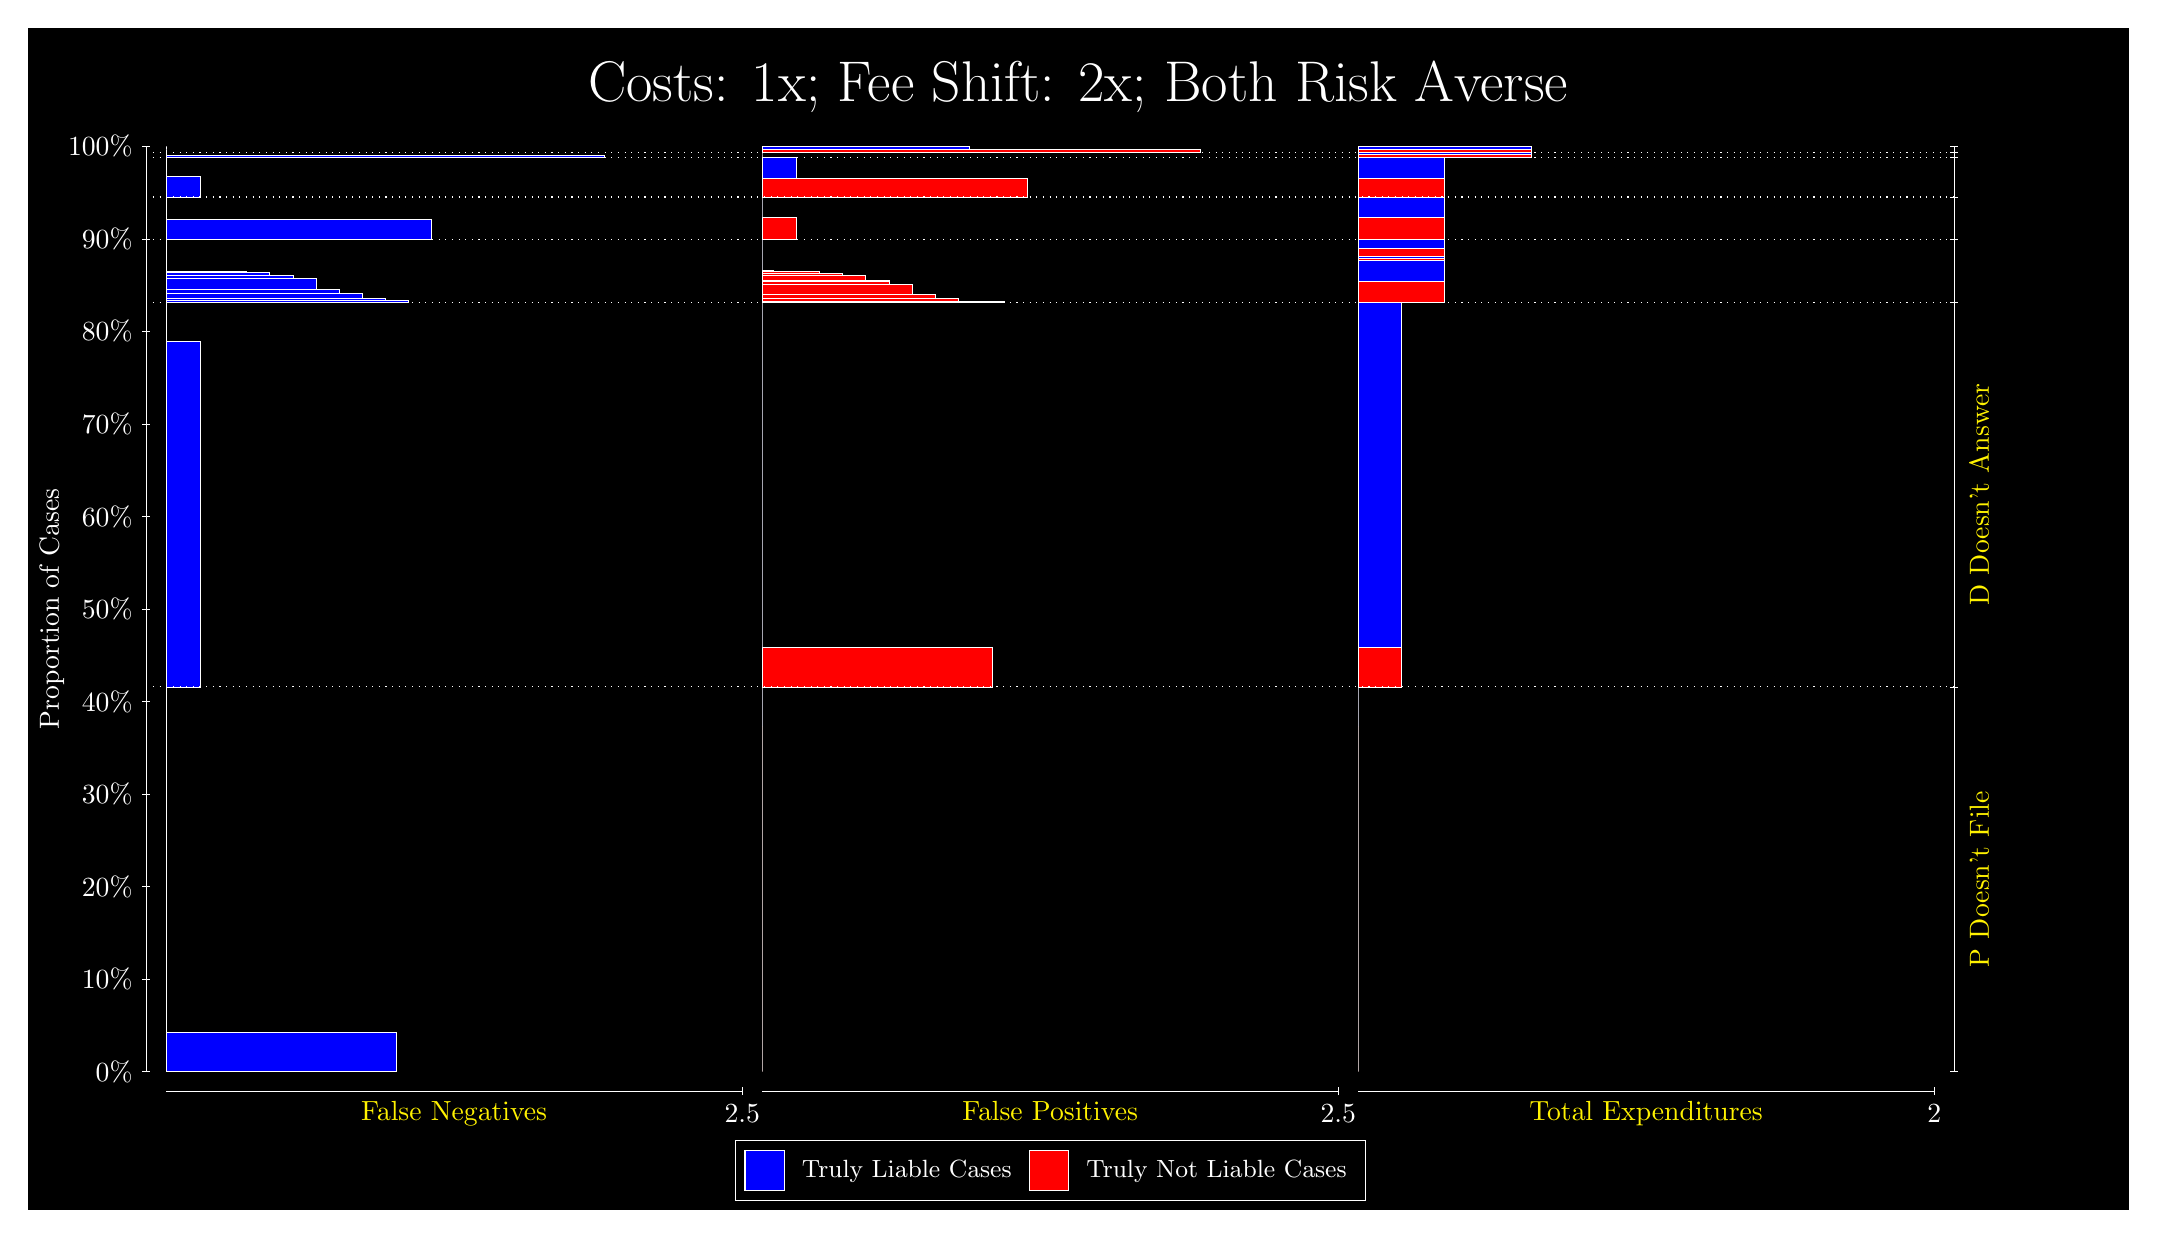
\begin{tikzpicture}
\draw[fill=black] (0,0) rectangle (26.667,15);
\draw[text=white] (0,13.5) rectangle (26.667,15) node[midway] {\huge Costs: 1x; Fee Shift: 2x; Both Risk Averse};
\draw[white, very thin] (1.5,1.75) -- (1.5,13.5);
\node[rotate=90, text=white, anchor=center] at (0.3, 7.625) {Proportion of Cases};
\draw[white, very thin] (1.45,1.75) -- (1.55,1.75);
\node[text=white, anchor=east] at (1.45, 1.75) {0\%};
\draw[white, very thin] (1.45,2.925) -- (1.55,2.925);
\node[text=white, anchor=east] at (1.45, 2.925) {10\%};
\draw[white, very thin] (1.45,4.1) -- (1.55,4.1);
\node[text=white, anchor=east] at (1.45, 4.1) {20\%};
\draw[white, very thin] (1.45,5.275) -- (1.55,5.275);
\node[text=white, anchor=east] at (1.45, 5.275) {30\%};
\draw[white, very thin] (1.45,6.45) -- (1.55,6.45);
\node[text=white, anchor=east] at (1.45, 6.45) {40\%};
\draw[white, very thin] (1.45,7.625) -- (1.55,7.625);
\node[text=white, anchor=east] at (1.45, 7.625) {50\%};
\draw[white, very thin] (1.45,8.8) -- (1.55,8.8);
\node[text=white, anchor=east] at (1.45, 8.8) {60\%};
\draw[white, very thin] (1.45,9.975) -- (1.55,9.975);
\node[text=white, anchor=east] at (1.45, 9.975) {70\%};
\draw[white, very thin] (1.45,11.15) -- (1.55,11.15);
\node[text=white, anchor=east] at (1.45, 11.15) {80\%};
\draw[white, very thin] (1.45,12.325) -- (1.55,12.325);
\node[text=white, anchor=east] at (1.45, 12.325) {90\%};
\draw[white, very thin] (1.45,13.5) -- (1.55,13.5);
\node[text=white, anchor=east] at (1.45, 13.5) {100\%};

\draw[white, very thin] (24.457,1.75) -- (24.457,13.5);
\draw[white, very thin] (24.407,1.75) -- (24.507,1.75);
\node[anchor=west] at (24.407, 1.75) {};
\draw[white, very thin] (24.407,6.6358) -- (24.507,6.6358);
\node[anchor=west] at (24.407, 6.6358) {};
\draw[white, very thin] (24.407,11.521) -- (24.507,11.521);
\node[anchor=west] at (24.407, 11.521) {};
\draw[white, very thin] (24.407,12.314) -- (24.507,12.314);
\node[anchor=west] at (24.407, 12.314) {};
\draw[white, very thin] (24.407,12.856) -- (24.507,12.856);
\node[anchor=west] at (24.407, 12.856) {};
\draw[white, very thin] (24.407,13.355) -- (24.507,13.355);
\node[anchor=west] at (24.407, 13.355) {};
\draw[white, very thin] (24.407,13.426) -- (24.507,13.426);
\node[anchor=west] at (24.407, 13.426) {};
\draw[white, very thin] (24.407,13.5) -- (24.507,13.5);
\node[anchor=west] at (24.407, 13.5) {};

\draw[white, very thin, fill=blue] (1.75,1.75) rectangle (4.6775,2.2488);
\draw[white, very thin, fill=red] (1.75,2.2488) rectangle (1.75,6.6358);
\draw[white, very thin, fill=blue] (1.75,6.6358) rectangle (2.1891,11.022);
\draw[white, very thin, fill=red] (1.75,11.022) rectangle (1.75,11.521);
\draw[white, very thin, fill=blue] (1.75,11.521) rectangle (4.8239,11.546);
\draw[white, very thin, fill=blue] (1.75,11.546) rectangle (4.5312,11.573);
\draw[white, very thin, fill=blue] (1.75,11.573) rectangle (4.2384,11.637);
\draw[white, very thin, fill=blue] (1.75,11.637) rectangle (3.9457,11.685);
\draw[white, very thin, fill=blue] (1.75,11.685) rectangle (3.6529,11.819);
\draw[white, very thin, fill=blue] (1.75,11.819) rectangle (3.3602,11.86);
\draw[white, very thin, fill=blue] (1.75,11.86) rectangle (3.0674,11.899);
\draw[white, very thin, fill=blue] (1.75,11.899) rectangle (2.7746,11.908);
\draw[white, very thin, fill=blue] (1.75,11.908) rectangle (2.4819,11.916);
\draw[white, very thin, fill=red] (1.75,11.916) rectangle (1.75,12.314);
\draw[white, very thin, fill=blue] (1.75,12.314) rectangle (5.1167,12.574);
\draw[white, very thin, fill=red] (1.75,12.574) rectangle (1.75,12.856);
\draw[white, very thin, fill=blue] (1.75,12.856) rectangle (2.1891,13.117);
\draw[white, very thin, fill=red] (1.75,13.117) rectangle (1.75,13.355);
\draw[white, very thin, fill=blue] (1.75,13.355) rectangle (7.3123,13.387);
\draw[white, very thin, fill=red] (1.75,13.387) rectangle (1.75,13.426);
\draw[white, very thin, fill=red] (1.75,13.426) rectangle (1.75,13.459);
\draw[white, very thin, fill=blue] (1.75,13.459) rectangle (1.75,13.5);
\draw[white, very thin, fill=red] (9.3189,1.75) rectangle (9.3189,6.137);
\draw[white, very thin, fill=blue] (9.3189,6.137) rectangle (9.3189,6.6358);
\draw[white, very thin, fill=red] (9.3189,6.6358) rectangle (12.246,7.134);
\draw[white, very thin, fill=blue] (9.3189,7.134) rectangle (9.3189,11.521);
\draw[white, very thin, fill=red] (9.3189,11.521) rectangle (12.393,11.527);
\draw[white, very thin, fill=red] (9.3189,11.527) rectangle (12.1,11.536);
\draw[white, very thin, fill=red] (9.3189,11.536) rectangle (11.807,11.576);
\draw[white, very thin, fill=red] (9.3189,11.576) rectangle (11.515,11.616);
\draw[white, very thin, fill=red] (9.3189,11.616) rectangle (11.222,11.75);
\draw[white, very thin, fill=red] (9.3189,11.75) rectangle (10.929,11.787);
\draw[white, very thin, fill=red] (9.3189,11.787) rectangle (10.929,11.798);
\draw[white, very thin, fill=red] (9.3189,11.798) rectangle (10.636,11.862);
\draw[white, very thin, fill=red] (9.3189,11.862) rectangle (10.344,11.889);
\draw[white, very thin, fill=red] (9.3189,11.889) rectangle (10.051,11.918);
\draw[white, very thin, fill=blue] (9.3189,11.918) rectangle (9.4652,11.926);
\draw[white, very thin, fill=blue] (9.3189,11.926) rectangle (9.3189,12.314);
\draw[white, very thin, fill=red] (9.3189,12.314) rectangle (9.758,12.596);
\draw[white, very thin, fill=blue] (9.3189,12.596) rectangle (9.3189,12.856);
\draw[white, very thin, fill=red] (9.3189,12.856) rectangle (12.686,13.094);
\draw[white, very thin, fill=blue] (9.3189,13.094) rectangle (9.758,13.355);
\draw[white, very thin, fill=red] (9.3189,13.355) rectangle (9.3189,13.394);
\draw[white, very thin, fill=blue] (9.3189,13.394) rectangle (9.3189,13.426);
\draw[white, very thin, fill=red] (9.3189,13.426) rectangle (14.881,13.459);
\draw[white, very thin, fill=blue] (9.3189,13.459) rectangle (11.954,13.5);
\draw[white, very thin, fill=red] (16.888,1.75) rectangle (16.888,6.137);
\draw[white, very thin, fill=blue] (16.888,6.137) rectangle (16.888,6.6358);
\draw[white, very thin, fill=red] (16.888,6.6358) rectangle (17.437,7.134);
\draw[white, very thin, fill=blue] (16.888,7.134) rectangle (17.437,11.521);
\draw[white, very thin, fill=red] (16.888,11.521) rectangle (17.986,11.787);
\draw[white, very thin, fill=blue] (16.888,11.787) rectangle (17.986,12.054);
\draw[white, very thin, fill=red] (16.888,12.054) rectangle (17.986,12.083);
\draw[white, very thin, fill=blue] (16.888,12.083) rectangle (17.986,12.108);
\draw[white, very thin, fill=red] (16.888,12.108) rectangle (17.986,12.211);
\draw[white, very thin, fill=blue] (16.888,12.211) rectangle (17.986,12.314);
\draw[white, very thin, fill=red] (16.888,12.314) rectangle (17.986,12.596);
\draw[white, very thin, fill=blue] (16.888,12.596) rectangle (17.986,12.856);
\draw[white, very thin, fill=red] (16.888,12.856) rectangle (17.986,13.094);
\draw[white, very thin, fill=blue] (16.888,13.094) rectangle (17.986,13.355);
\draw[white, very thin, fill=red] (16.888,13.355) rectangle (19.083,13.394);
\draw[white, very thin, fill=blue] (16.888,13.394) rectangle (19.083,13.426);
\draw[white, very thin, fill=red] (16.888,13.426) rectangle (19.083,13.459);
\draw[white, very thin, fill=blue] (16.888,13.459) rectangle (19.083,13.5);
\draw[white, dotted] (1.5,6.6358) -- (24.457,6.6358);
\draw[white, dotted] (1.5,11.521) -- (24.457,11.521);
\draw[white, dotted] (1.5,12.314) -- (24.457,12.314);
\draw[white, dotted] (1.5,12.856) -- (24.457,12.856);
\draw[white, dotted] (1.5,13.355) -- (24.457,13.355);
\draw[white, dotted] (1.5,13.426) -- (24.457,13.426);
\draw[white, very thin] (1.75,1.5) -- (9.0689,1.5);
\node[text=yellow, anchor=north] at (5.4094, 1.5) {False Negatives};
\draw[white, very thin] (9.0689,1.45) -- (9.0689,1.55);
\node[text=white, anchor=north] at (9.0689, 1.45) {2.5};

\draw[white, very thin] (9.3189,1.5) -- (16.638,1.5);
\node[text=yellow, anchor=north] at (12.978, 1.5) {False Positives};
\draw[white, very thin] (16.638,1.45) -- (16.638,1.55);
\node[text=white, anchor=north] at (16.638, 1.45) {2.5};

\draw[white, very thin] (16.888,1.5) -- (24.207,1.5);
\node[text=yellow, anchor=north] at (20.547, 1.5) {Total Expenditures};
\draw[white, very thin] (24.207,1.45) -- (24.207,1.55);
\node[text=white, anchor=north] at (24.207, 1.45) {2};

\node[text=yellow, centered, rotate=90] at (24.777, 4.1929) {P Doesn't File};
\node[text=yellow, centered, rotate=90] at (24.777, 9.0782) {D Doesn't Answer};






\draw (12.978300999999998,1.5) node[draw=none] (baseCoordinate) {};
\begin{scope}[align=center]
        \matrix[scale=0.5, draw=white, below=0.5cm of baseCoordinate, nodes={draw}, column sep=0.1cm]{
            \node[rectangle, draw, minimum width=0.5cm, minimum height=0.5cm, fill=blue] {}; &
            \node[draw=none, font=\small, text=white] (B) {Truly Liable Cases}; &
            \node[rectangle, draw, minimum width=0.5cm, minimum height=0.5cm, fill=red] {}; &
            \node[draw=none, font=\small, text=white] (B) {Truly Not Liable Cases}; \\
            };
\end{scope}

\end{tikzpicture}
\end{document}